\documentclass[14pt]{beamer}\beamertemplatenavigationsymbolsempty
%\documentclass[a4paper]{scrartcl}\usepackage{beamerarticle}

\usepackage[T1]{fontenc}
\usepackage[utf8]{inputenc}
\usepackage{default}
\usepackage{hyperref}
\usepackage[english]{babel}
\usepackage{amsmath}
\usepackage{lmodern}
\usepackage{graphicx}
\usepackage{listings}
\usepackage[backend=biber,citestyle=alphabetic,bibstyle=din]{biblatex}
\bibliography{accelerate}

\lstset{basicstyle=\scriptsize\ttfamily,
        breaklines=false,
%        frame=single,
%        keywordstyle=\ttfamily,
        language=llvm}

\usetheme{Pittsburgh}

\title{Generating LLVM IR using
Template Meta Programming}
\author{Timo von Holtz}
\date{\today}
%\institute{Institut für Informatik}
\setbeamertemplate{footline}[frame number]

\newcommand{\executeIffilenewer}[3]{
 \ifnum\pdfstrcmp{\pdffilemoddate{#1}}
 {\pdffilemoddate{#2}}>0
 {\immediate\write18{#3}}\fi
}
\newcommand{\includesvg}[2][]{
 \executeIffilenewer{#2.svg}{#2.pdf}
 {inkscape -z -D --file=#2.svg --export-pdf=#2.pdf}
 \includegraphics[#1]{#2.pdf}
}

\begin{document}
\maketitle

\section{Introduction}
\subsection{Accelerate}
\begin{frame}
 \frametitle{Accelerate}
 \begin{itemize}
\item Embedded array language
\item Compiled online
\item CUDA backend
\end{itemize}
\end{frame}

\begin{frame}
 \frametitle{LLVM Backend}
\begin{itemize}
\item CPU/GPU
\item no external process
\item incomplete
\end{itemize}
\end{frame}
\subsection{LLVM}
\begin{frame}
 \frametitle{Overview LLVM}
\begin{itemize}
\item Compiler library
\item Portable
\item Haskell bindings (llvm-general)
\item Auto-Vectorization
\item Static Single Assignment (SSA)
\end{itemize}
\end{frame}

\begin{frame}[fragile]
 \frametitle{Code Example LLVM}
\begin{columns}[c]
\column{.3\textwidth}
\begin{lstlisting}[language=C]
int abs(int x) {
    int res;
    if (x>0) {
        res = x;
    } else {
        res = -x;
    }
    return res;
}
\end{lstlisting}
\column{.7\textwidth}
\begin{lstlisting}[language=llvm]
define i32 @abs(i32 %x) {
entry:
  %1 = icmp sgt i32 %x, 0
  br i1 %1, label %then, label %else

then:              ; preds = %entry
  br label %5

else:              ; preds = %entry
  %4 = sub nsw i32 0, %x
  br label %5

end:               ; preds = %else, %then
  %res.0 = phi i32 [ %x, %then ],
                   [ %4, %else ]
  ret i32 %res.0
}
\end{lstlisting}
\end{columns}
\end{frame}

\begin{frame}
\frametitle{llvm-general}
\begin{itemize}
\item uses ADT to represent syntax tree
\item translates from and to C++ Objects
\item exposes Optimizer/JIT compiler
\end{itemize}
\end{frame}

\section{Code Generation}
\subsection{Quasiquoting}
\begin{frame}[fragile]
 \frametitle{Quasiquoting}
\begin{lstlisting}[language=llvm]
abs :: Global
abs = [llg|
  define i32 @abs(i32 %x) {
  entry:
    %1 = icmp sgt i32 %x, 0
    br i1 %1, label %end, label %else

  else:
    %4 = sub nsw i32 0, %x
    br label %5

  end:
    %res.0 = phi i32 [ %x, %entry ],
                     [ %4, %else ]
    ret i32 %res.0
  }
  |]
\end{lstlisting}
\end{frame}
\subsection{Control Structures (1st attempt)}
\begin{frame}[fragile]
 \frametitle{Control Structures}
\begin{lstlisting}
i32 foo(i32 %m, i32 %n) {
  entry:
    br label %for

  for:
    for i32 %i in %m to %n with i32 [ 0, %entry ] as %j,
                                              label %end {
        %k = add i32 %i, %j
        ret i32 %k
    }

  end:
    ret i32 %j
}
\end{lstlisting}
\end{frame}
\subsection{Control Structures (2nd attempt)}
\begin{frame}[fragile]
 \frametitle{Control Structures}
\begin{lstlisting}
i32 foo(i32 %m, i32 %n) {
  entry:
    br label %for

  for:
    for i32 %i in %m to %n with i32 [ 0, %entry ] as %j {
        %k = add i32 %i, %j
        ret i32 %k
    }

  end:
    ret i32 %j
}
\end{lstlisting}
\end{frame}
\subsection{Control Structures (SSA)}
\begin{frame}[fragile]
 \frametitle{Control Structures}
\begin{lstlisting}
define i64 @foo(i64 %start, i64 %end) {
  entry:
    %x = i64 0

  for:
    for i64 %i in %start to %end {
        %x = add i64 %i, %x
    }

  exit:
    ret i64 %x
}
\end{lstlisting}
\end{frame}
\subsection{SSA}
\begin{frame}
 \frametitle{SSA}
 \nocite{braun13simple}
 \printbibliography
\end{frame}

\begin{frame}[fragile]
\frametitle{Local value numbering}
\begin{lstlisting}[language=ruby]
writeVariable(variable, block, value):
    currentDef[variable][block] <- value

readVariable(variable, block):
    if currentDef[variable] contains block:
        # local value numbering
        return currentDef[variable][block]
    # global value numbering
    return readVariableRecursive(variable, block)
\end{lstlisting}
\end{frame}

\begin{frame}[fragile]
\frametitle{Global value numbering}
\begin{lstlisting}[language=ruby]
readVariableRecursive(variable, block):
    if |block.preds| = 0:
        # First block
        val <- variable
    else:
        # Break potential cycles with operandless phi
        val <- new Phi(block)
        writeVariable(variable, block, val)
    writeVariable(variable, block, val)
    return val
\end{lstlisting}
\end{frame}

\begin{frame}[fragile]
\begin{lstlisting}
define i64 @foo(i64 %start, i64 %end) {
entry:
  br label %for.head

for.head:                      ; preds = %n0, %entry
  %x.12 = phi i64 [ 0, %entry ], [ %x.6, %n0 ]
  %i.4 = phi i64 [ %start, %entry ], [ %i.9, %n0 ]
  %for.cond.3 = icmp slt i64 %i.4, %end
  br i1 %for.cond.3, label %n0, label %for.end

n0:                            ; preds = %for.head
  %x.6 = add i64 %i.4, %x.12
  %i.9 = add nuw nsw i64 %i.4, 1
  br label %for.head

for.end:                       ; preds = %for.head
  ret i64 %x.12
}
\end{lstlisting}
\end{frame}

\section{Benchmarks}
\begin{frame}
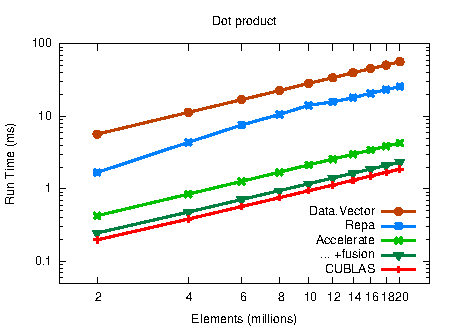
\includegraphics[width=\textwidth]{images/benchmarks/dotp/dotp}
\end{frame}

\begin{frame}
% \frametitle{Titel}
\begin{center}
\begin{tabular}{ll}
Step             & Time (ms)   \\ \hline
getTarget        & 0.098  \\
llvmOfAcc              & 0.0771 \\
startFunction    & 0.0403 \\
withContext      & 0.0879 \\
withModuleFromAST       & 6.8032 \\
withMachine      & 0.2997 \\
libinfo          & 0.0801 \\
optimizeModule   & 4.0379 \\
withMCJIT        & 0.05   \\
withModuleInEngine   & 0.2374 \\
getGlobalFunctions & 9.8508 \\
\end{tabular}
\end{center}
\end{frame}

\begin{frame}
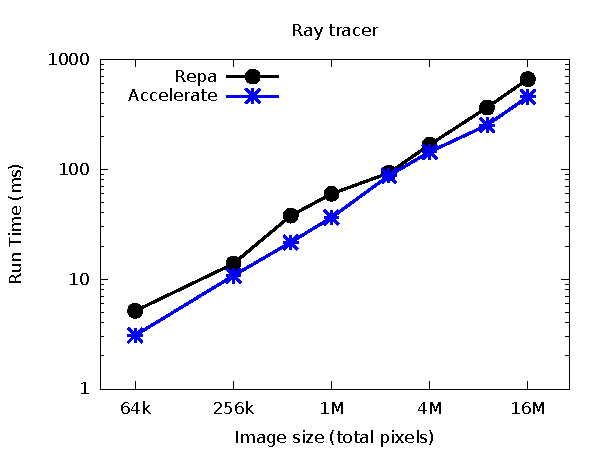
\includegraphics[width=\textwidth]{images/benchmarks/ray/ray}
\end{frame}

\begin{frame}
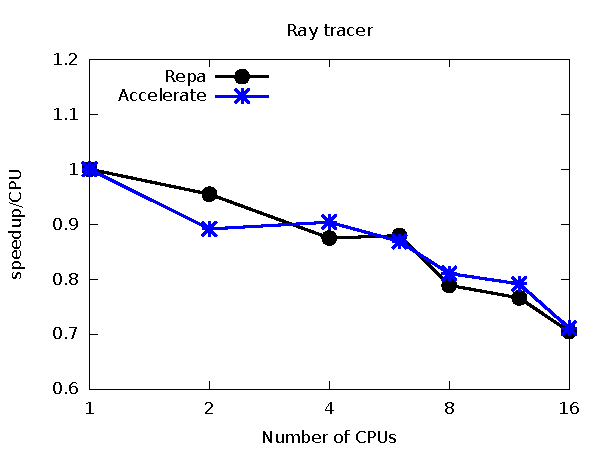
\includegraphics[width=\textwidth]{images/benchmarks/ray/ray-scale}
\end{frame}

\end{document}
